\documentclass[main.tex]{subfiles}

\begin{document}
\chapter{Parallelization of DFPT calculations}\label{ch:optimization_ph}

Calculations with the \texttt{PHonon} package are significantly more time intensive than \texttt{PWscf} calculations, so good parallelization is of the essence to make these calculations manageable.

\section{Optimal parallelization parameters for DFPT calculations}

The \texttt{PHonon} package offers the same three parallelization levels as the \texttt{PWscf} package, namely plane wave, k point and linear algebra parallelization.
Furthermore parallelization across q points (so called image parallelization) can be employed, this will be discussed separately in sec. \ref{sec:scaling_ph_images}.

\subsection{k point parallelization}

In a first step, the same k point parallelization benchmark as in sec. \ref{sub:scf_scaling_k_point} is run. This is pictured in fig. \ref{fig:scaling_ph_nk_si}.

\begin{figure}[ht!]
    \centering
    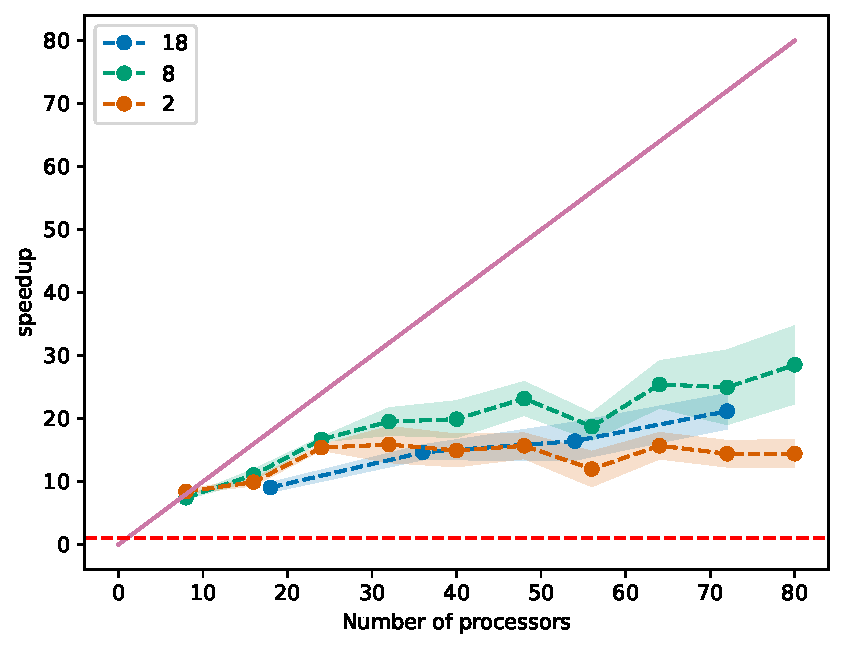
\includegraphics[width=0.8\textwidth]{plots_ph/si_ph_bench_nk_speedup.pdf}
    \caption{Scalability utilizing k-point parallelization for the Si benchmarking system with three sizes of processor pools, \emph{\QE compiled with \gls{oneapi} 2021.4, \texttt{nd 1}}}
    \label{fig:scaling_ph_nk_si}
\end{figure}
Interestingly, the results from sec. \ref{sub:scf_scaling_k_point} is not reproduced here: the smallest pool size of 2 is not the fastest, but instead it is pool size 8.

\begin{figure}[ht!]
    \centering
    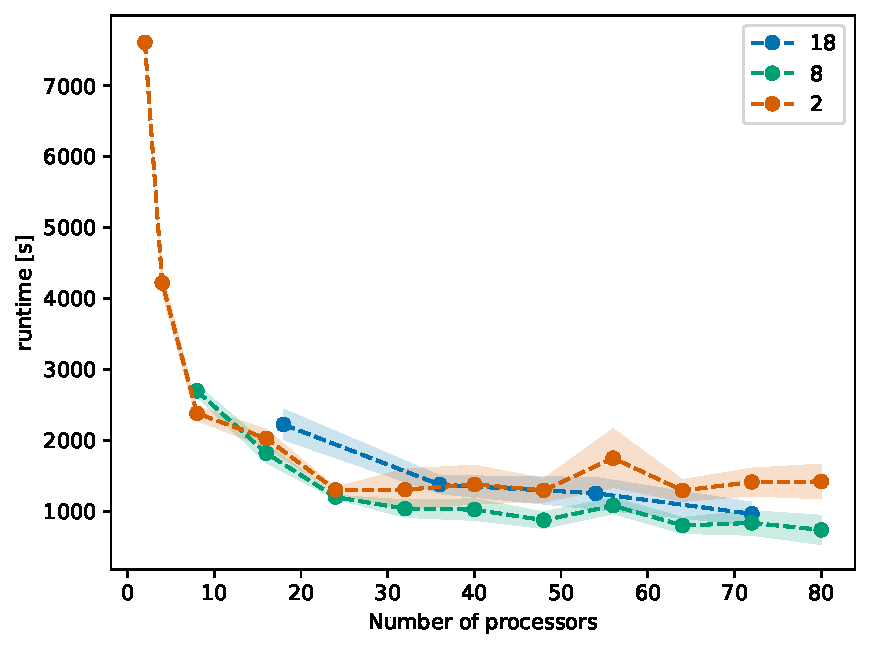
\includegraphics[width=0.8\textwidth]{plots_ph/si_ph_bench_nk_absolute.pdf}
    \caption{Absolute runtime for the scalability test utilizing k-point parallelization for the Si benchmarking system with three sizes of processor pools, \emph{\QE compiled with \gls{oneapi} 2021.4, \texttt{nd 1}}}
    \label{fig:scaling_ph_nk_si_absolute}
\end{figure}

\subsection{Linear algebra parallelization}

\section{Image parallelization}\label{sec:scaling_ph_images}

\todo{Better introduction}
When using image parallelization, \QE outputs a separate time report for every image, so one step is added to the analysis:
The total runtime of a calculation is determined by the longest running image, so speedup will be calculated using that value, but another important measure to evaluate is variation of times between images.
This is pictured in fig. \ref{fig:scaling_ph_ni_poolsize_8_si}.

\begin{figure}[ht!]
    \centering
    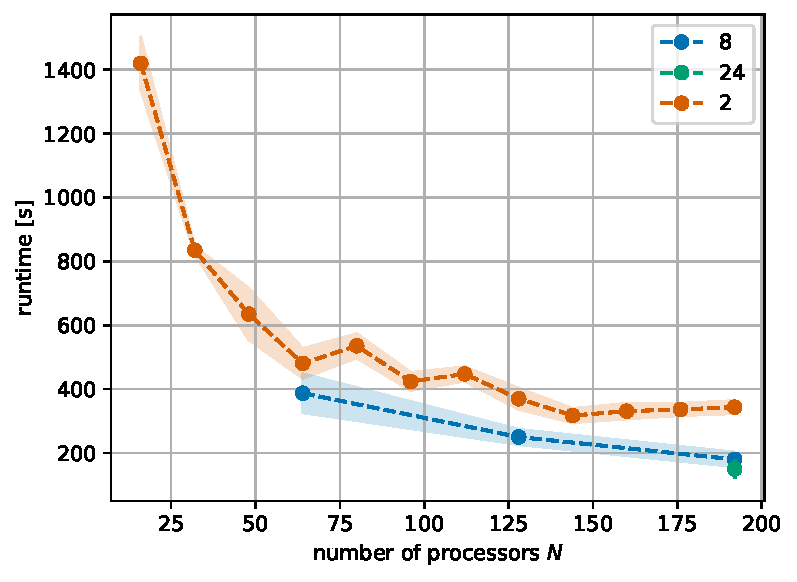
\includegraphics[width=0.8\textwidth]{plots_ph/si_ph_poolsize_8_images_distribution.pdf}
    \caption{Average runtime across images for the scalability test utilizing image and k point parallelization on the Si benchmarking system with three values of \emph{\texttt{ni}}, \emph{\QE compiled with \gls{oneapi} 2021.4, \texttt{nk, ni} chosen such that poolsize = 8, \texttt{nd 1}}}
    \label{fig:scaling_ph_ni_poolsize_8_si_distribution}
\end{figure}
As the times between images don't vary much, good load balancing between images can be assumed for the silicon benchmarking system.

With the maximum time across images, speedup is then calculated, pictured in fig. \ref{fig:scaling_ph_ni_poolsize_8_si}.

\begin{figure}[ht!]
    \centering
    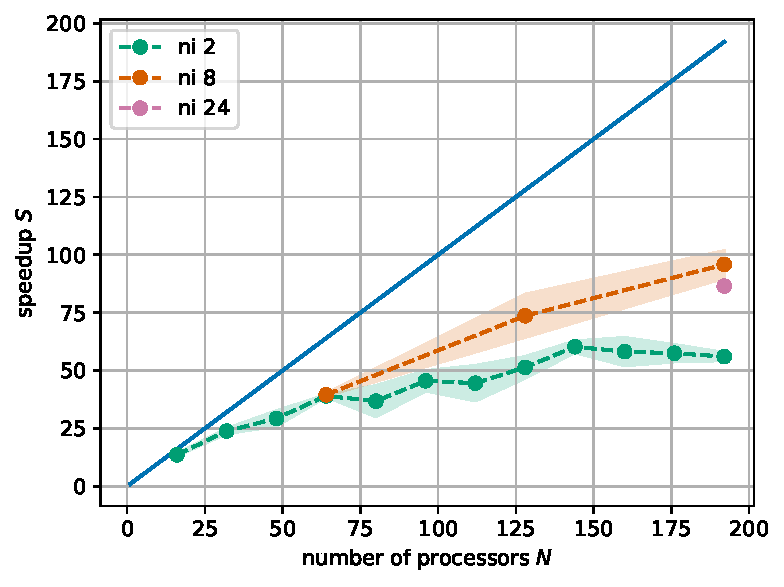
\includegraphics[width=0.8\textwidth]{plots_ph/si_ph_poolsize_8_bench_ni_speedup.pdf}
    \caption{Speedup calculated from the longest running image for the scalability test utilizing image and k point parallelization on the Si benchmarking system with three values of \emph{\texttt{ni}}, \emph{\QE compiled with \gls{oneapi} 2021.4, \texttt{nk, ni} chosen such that poolsize = 8, \texttt{nd 1}}}
    \label{fig:scaling_ph_ni_poolsize_8_si}
\end{figure}


\begin{figure}[ht!]
    \centering
    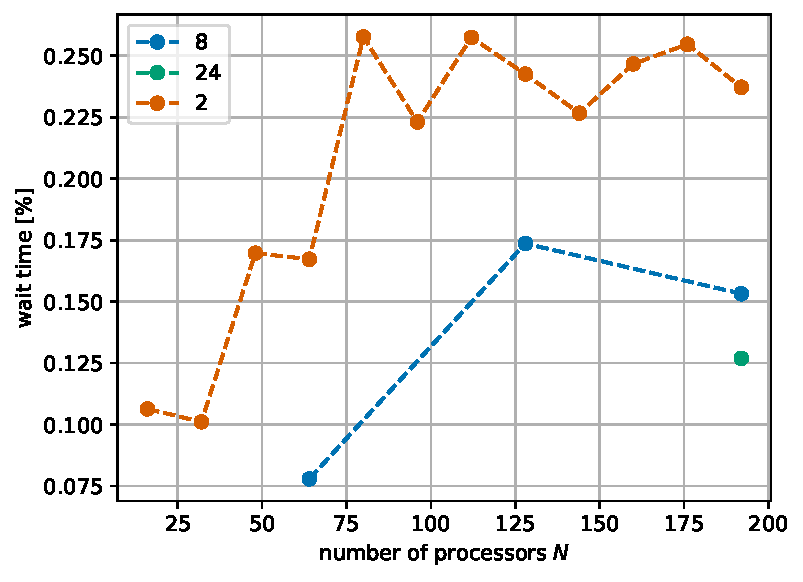
\includegraphics[width=0.8\textwidth]{plots_ph/si_ph_poolsize_8_bench_ni_wait.pdf}
    \caption{Wait time calculated from the longest running image for the scalability test utilizing image and k point parallelization on the Si benchmarking system with three values of \emph{\texttt{ni}}, \emph{\QE compiled with \gls{oneapi} 2021.4, \texttt{nk, ni} chosen such that poolsize = 8, \texttt{nd 1}}}
    \label{fig:scaling_ph_ni_poolsize_8_si_wait}
\end{figure}

\section{Conclusion: Parameters for optimal scaling}

\end{document}